\documentclass[]{report}
\usepackage{amsmath}
\usepackage{amssymb}
\usepackage[english]{babel}
\usepackage[utf8]{inputenc}
\usepackage[T1]{fontenc}
\usepackage{euler}

\usepackage[inner=0cm,outer=0cm,top=0cm,bottom=0cm,paperwidth=10cm,paperheight=9.8cm]{geometry}

\usepackage{tikz,pgfplots}
\usetikzlibrary{positioning}
\usetikzlibrary{decorations.pathmorphing}

\begin{document}

\centering
\begin{tikzpicture}
	%\draw[help lines,xstep=1,ystep=1] (0,0) grid (10,10);
	\node[anchor=south west,inner sep=0] at (0,0) {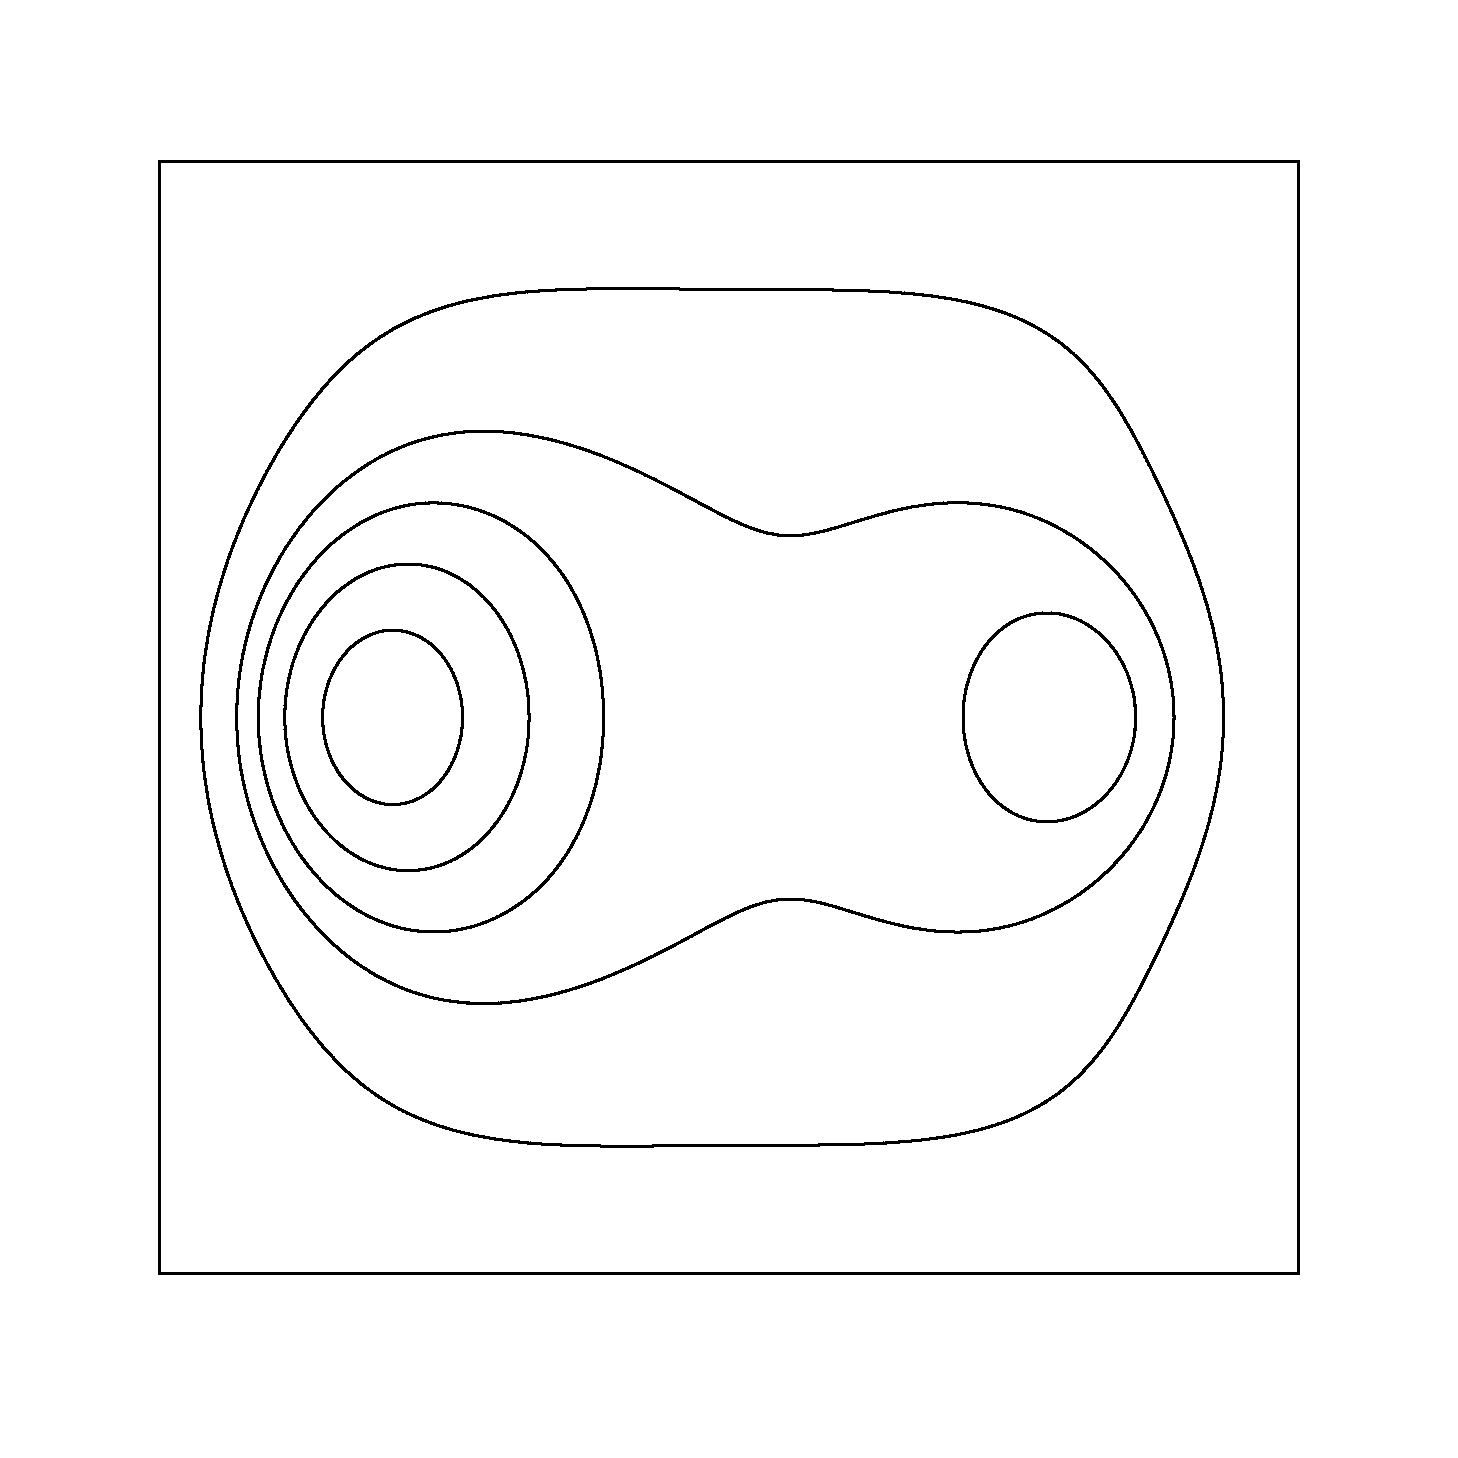
\includegraphics[width=10cm]{out}};
	
	\fill[fill=black] (2.1 ,4.9) circle (0.1) node[left] {\large $A$};
	\fill[fill=black] (2.57,4.9) circle (0.1);
	\fill[fill=black] (3.05,4.9) circle (0.1);
	\fill[fill=black] (3.53,4.9) circle (0.1);
	\fill[fill=black] (4   ,4.9) circle (0.1);
	\fill[fill=black] (4.95,4.9) circle (0.1) node[] (1) {};
	\fill[fill=black] (5.9 ,4.9) circle (0.1);
	\fill[fill=black] (6.85,4.9) circle (0.1);
	\fill[fill=black] (7.33,4.9) circle (0.1);
	\fill[fill=black] (7.8 ,4.9) circle (0.1) node[right] {\large $B$};
	\draw[dashed, thick] (2.1,4.9) -- (7.8,4.9);
	\node[label=below:\large$s$] at (4.5,5.1) {};
	\node[anchor=west] (w) at (5,5.5) {\large windows};
	\draw[] (1) -- (w);
\end{tikzpicture}
\end{document}